\documentclass[nopagenumber,9pt]{beamer}

\mode<presentation> {
  \usetheme[]{CambridgeUS}
  %\useoutertheme{shadow}
  \setbeamercovered{transparent}
  \usecolortheme{seahorse}
%\usecolortheme{sidebartab}
%  \usefonttheme{structurebold}
  \useinnertheme{default}
\useinnertheme{rounded}
}
\usepackage{nicefrac}
\RequirePackage{amsmath,amsfonts,amsthm}

\usepackage{float}
\usepackage[english]{babel}
\usepackage{amsmath}
\usepackage[utf8]{inputenc}
\usepackage{times}
\usepackage{url}
\usepackage[T1]{fontenc}
%\usepackage{multirow}
\usepackage{color}
\newcommand{\mb}[1]{\mathbf{#1}}
\usepackage{graphicx}
\graphicspath{{./figure/}}

\definecolor{dgreen}{RGB}{139,172,100}

\hypersetup{
  colorlinks = true,
  linkcolor = black
}
\makeatletter
\let\@mycite\@cite
\def\@cite#1#2{{\hypersetup{linkcolor=dgreen}[{#1\if@tempswa , #2\fi}]}}
\makeatother

\usepackage[ruled,vlined]{algorithm2e}
\usepackage{xcolor,colortbl}
\usepackage{rotating}
\usepackage{multirow}

\usepackage{tikz}
\usepackage{ulem}

\usepackage{stmaryrd}
\newtheorem{proposition}{Proposition}

%appeler les macros
\usepackage{macros}

\title[Calibration]{Calibration of computer models}

%titre premiere page

\subtitle{Bayesian Calibration}

\author[P. Barbillon]{ Pierre \textsc{Barbillon}}
\bigskip

\date{Fall 2023}

\subject{Séminaire}



\AtBeginSection[] {
 \begin{frame}<beamer>
   \frametitle{Outline}
   \tableofcontents[currentsection]
  \end{frame}
}

\AtBeginSubsection[] {
\begin{frame}<beamer>
   \frametitle{Outline}
   \tableofcontents[currentsection,currentsubsection]
 \end{frame}
}


\begin{document}

\begin{frame}
\titlepage
%\includegraphics[scale=.12]{AgroParisTech_-_logo.PNG}
%\vspace{-1.5cm}
%\begin{flushright}
% \includegraphics[scale=.1]{Logotype-INRA-transparent.png}
% \end{flushright}
\vspace{-1cm}
\centering
\begin{tabular}{ccc}
 
\includegraphics[scale=.08]{LogoUPSaclay.jpg}&
  
\includegraphics[scale=1.3]{agrologo.png}&
   
\includegraphics[scale=.1]{LogoINRAE.jpg}
\end{tabular}


\end{frame}




 \section{A simple example}

\begin{frame}
\frametitle{Field data}
 
 \begin{itemize}
  \item Field data provided by physical experiments:
  $$\byexp=\yexp(\bxexp_1),\ldots,\yexp(\bxexp_{\nexp})\,,$$
\item[]
  \item $\nexp$ is small, $\bx_1,\ldots \bx_{\nexp} \in \mathcal{X}$ hard to set, sometimes uncontrollable, included in a small domain...
  \item[]
  \item Model:
  $$\yexp(\bxexp_i)=\zeta(\bxexp_i)+\epsilon(\bxexp_i)\,,$$
  where 
  \begin{itemize}
   \item $\zeta(\cdot)$ real physical process (unknown),
   \item $\epsilon(\bxexp_i)$ often assumed i.i.d. $\mathcal{N}(0,\sigma^2)$,
   \item $\sigma^2$ sometimes treated as known...
  \end{itemize}

  
  
  \end{itemize}

 
\end{frame}





\begin{frame}
 \frametitle{Relationship between the simulator and the data}

 for $i=1,\ldots, \nexp$,
\begin{itemize}
 \item if the simulator sufficiently represents the physical system:
 \begin{equation}
  \label{nodisc}
 \yexpi=f(\bxexp_i,\btheta^*)+\epsilon(\bxexp_i)\,,
 \end{equation}
 i.e. for the unknown value $\btheta=\btheta^*: f(\bx,\theta^*)=\zeta(\bx) $ for any $\bx\in \mathcal{X}$,

 \end{itemize}
 
 \end{frame}


 
  \begin{frame}
 \frametitle{A calibration example}

 \textbf{Prior:}\\
 prior distribution on unknown $\btheta$: $\pi(\cdot)$
 \\
 from expert judgment, past experiments...
 \\
 Possible choice $\pi(\btheta)=\mathcal{N}(\theta_0,\sigma_0^2)=\mathcal{N}(0.5,0.04)$.
 \\
 
 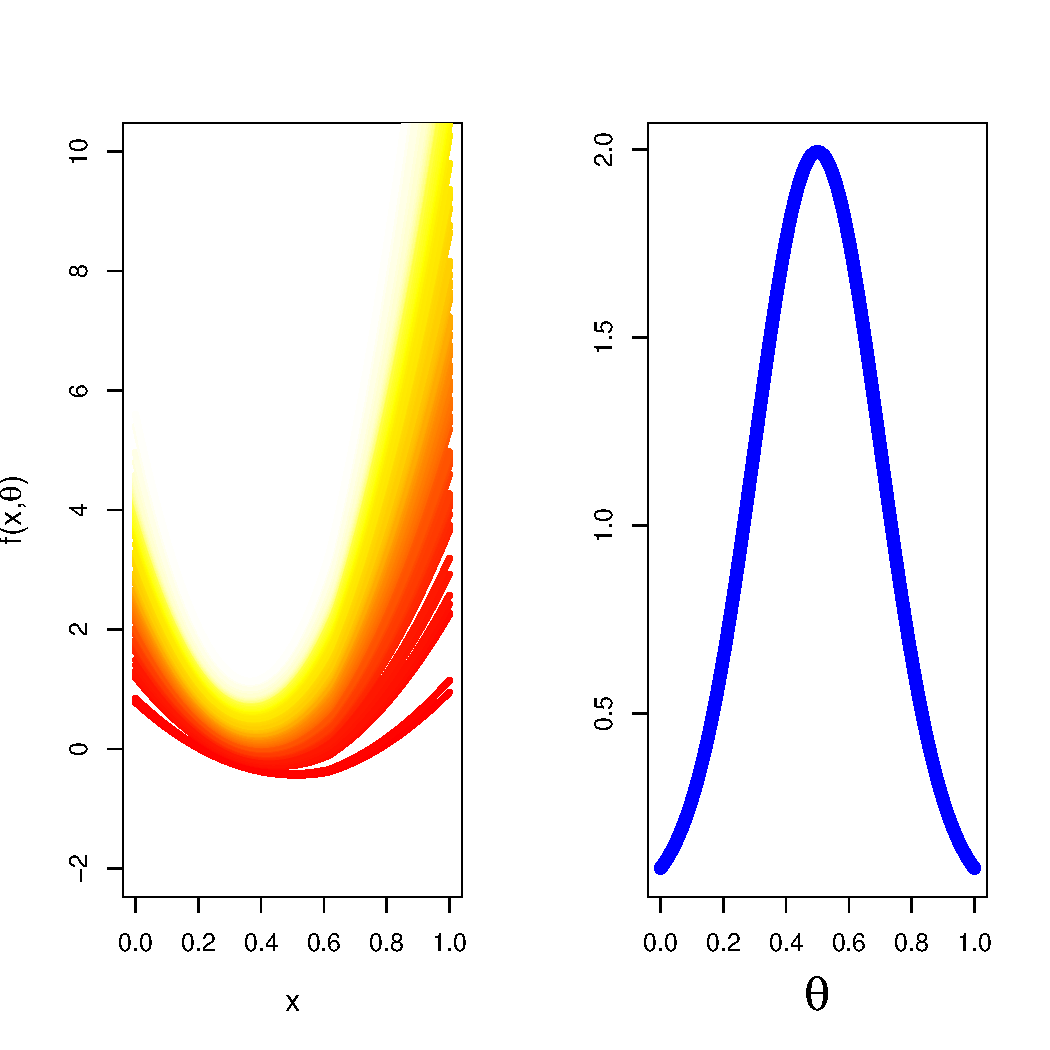
\includegraphics[width=1\textwidth,height=.5\textwidth]{prior.pdf}
 


 \end{frame}

 
 
 
 \begin{frame}
  \frametitle{A calibration example}
 \bigskip
 \textbf{Data:} \\
 Couples $(\bxexp_1,\yexp_1),\ldots,(\bxexp_{\nexp},\yexp_{\nexp})$
 from physical experiments.
 \\
 
 \bigskip
 \textbf{Posterior distribution:}\\
 \begin{eqnarray*}
\pi(\btheta|\byexp)&\propto& \mathcal{L}(\btheta|\byexp) \cdot \pi(\btheta)\\
&\propto&\exp\left( 
-\frac{1}{2\sigma^2}\sum_{i=1}^n (y(\bx_i)-f(\bx_i,\btheta))^2-\frac{1}{2\sigma_0^2}(\btheta-\btheta_0)^2
\right)  
 \end{eqnarray*}

 \begin{itemize}
  \item Analytical posterior if $\btheta\mapsto f(\bx,\btheta)$ is a linear map,
  \item Otherwise MH sampling to simulate according to the posterior distribution. \cite{robert1999monte}
 \end{itemize}


\end{frame}



\begin{frame}
 \frametitle{A calibration example}
 \textbf{Prior with data:}
%  \\
%  ($\theta^*=0.6$)\\
  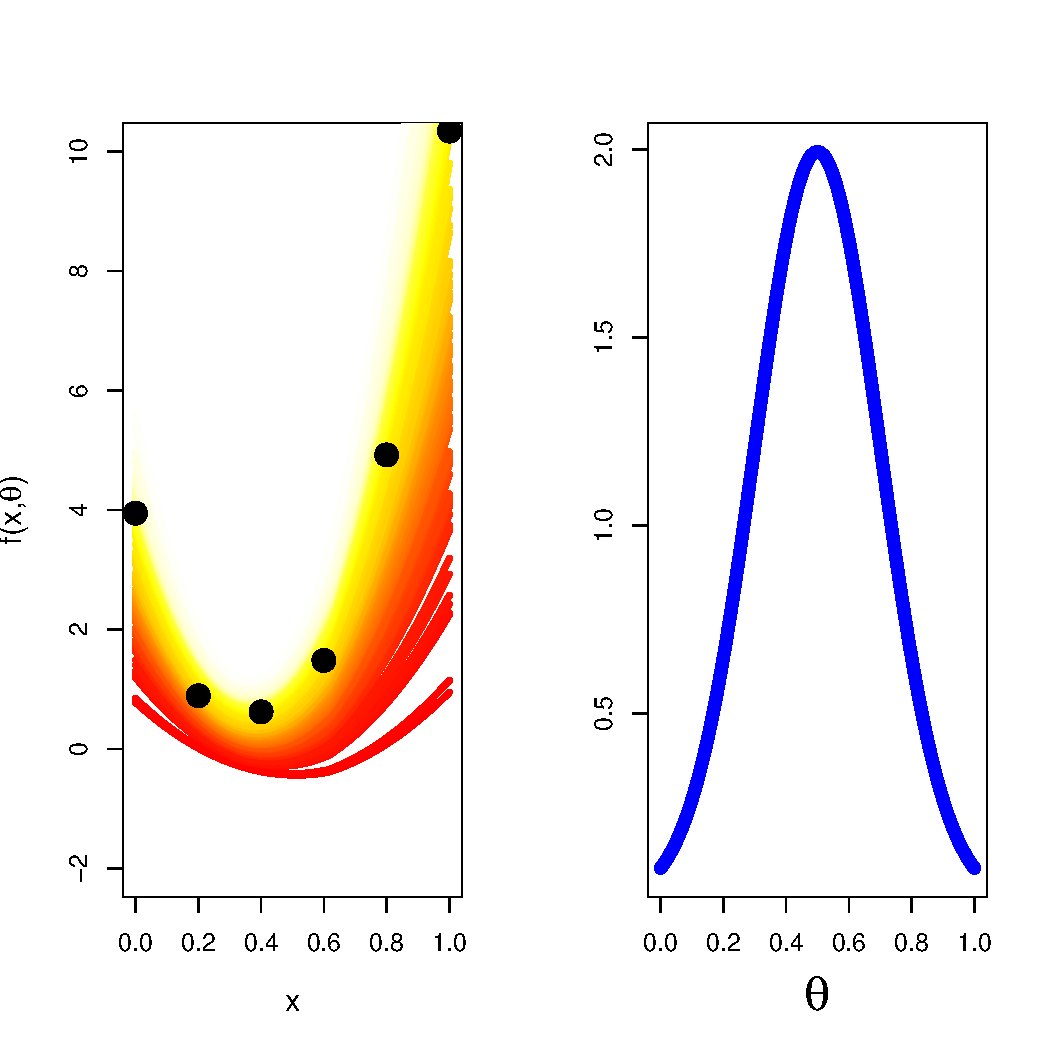
\includegraphics[width=.6\textwidth,height=.25\textwidth]{priordata.pdf}
 \\
 
 \bigskip
 \begin{scriptsize}
 
 \begin{center}
 $\Downarrow$
 Metropolis-Hastings algorithm $\Downarrow$
 \\
 \bigskip
  
 \end{center}

 \end{scriptsize}
 
 \textbf{Posterior on $\theta$:}
 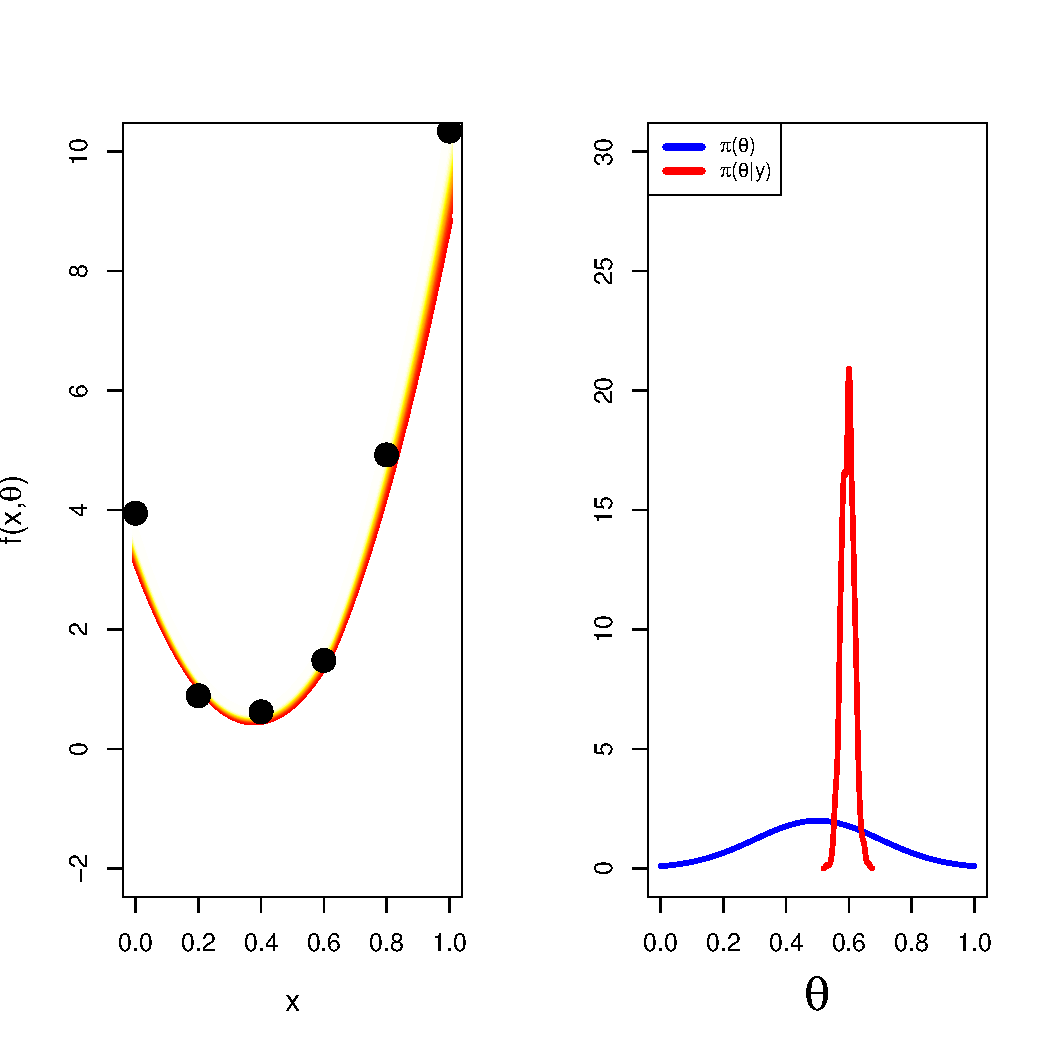
\includegraphics[width=.6\textwidth,height=.25\textwidth]{calibbonpriorsigconnu.pdf}
 
\end{frame}




\begin{frame}
 \frametitle{More details on the MH algorithm}
 
 \textbf{Initialisation:}\\
 $\btheta^0$ chosen.
 
 \bigskip
 
 \textbf{Update:}\\
 iterations $t=1,\ldots,$
\begin{enumerate}
 \item Proposal: $\tilde\btheta^{t+1}=\btheta^t+\mathcal{N}(0,\tau^2)$.
 \item Compute
 $$\alpha(\btheta^t,\tilde\btheta^{t+1})=\frac{\pi(\tilde\btheta^{t+1}|\byexp)}{\pi(\btheta^{t}|\byexp)}$$
 \item Acceptation:
 $$\btheta^{t+1}=\left\{\begin{array}{ll}
                       \tilde\btheta^{t+1}  & \text{with probability } \alpha(\btheta^t,\tilde\btheta^{t+1})\\
                       \btheta^t & \text{otherwise.}
                      \end{array}
 \right.$$
\end{enumerate}
 
 Note that the ratio $\alpha(\btheta^t,\tilde\btheta^{t+1})$
needs several computations of $f(\bx,\btheta)$ at each step
 since $$\pi(\btheta|\byexp)\propto
 \exp\left( 
-\frac{1}{2\sigma^2}\sum_{i=1}^n (\yexpi-f(\bxexp_i,\btheta))^2-\frac{1}{2\sigma_0^2}(\btheta-\btheta_0)^2
\right)  \,.$$
 
 
 
\end{frame}

\begin{frame}
 \frametitle{Unknown $\sigma^2$}
 
 \begin{itemize}
  \item  prior distribution on $\sigma^2$: $\pi(\sigma^2)=\mathcal{IG}(5,2)$\\
  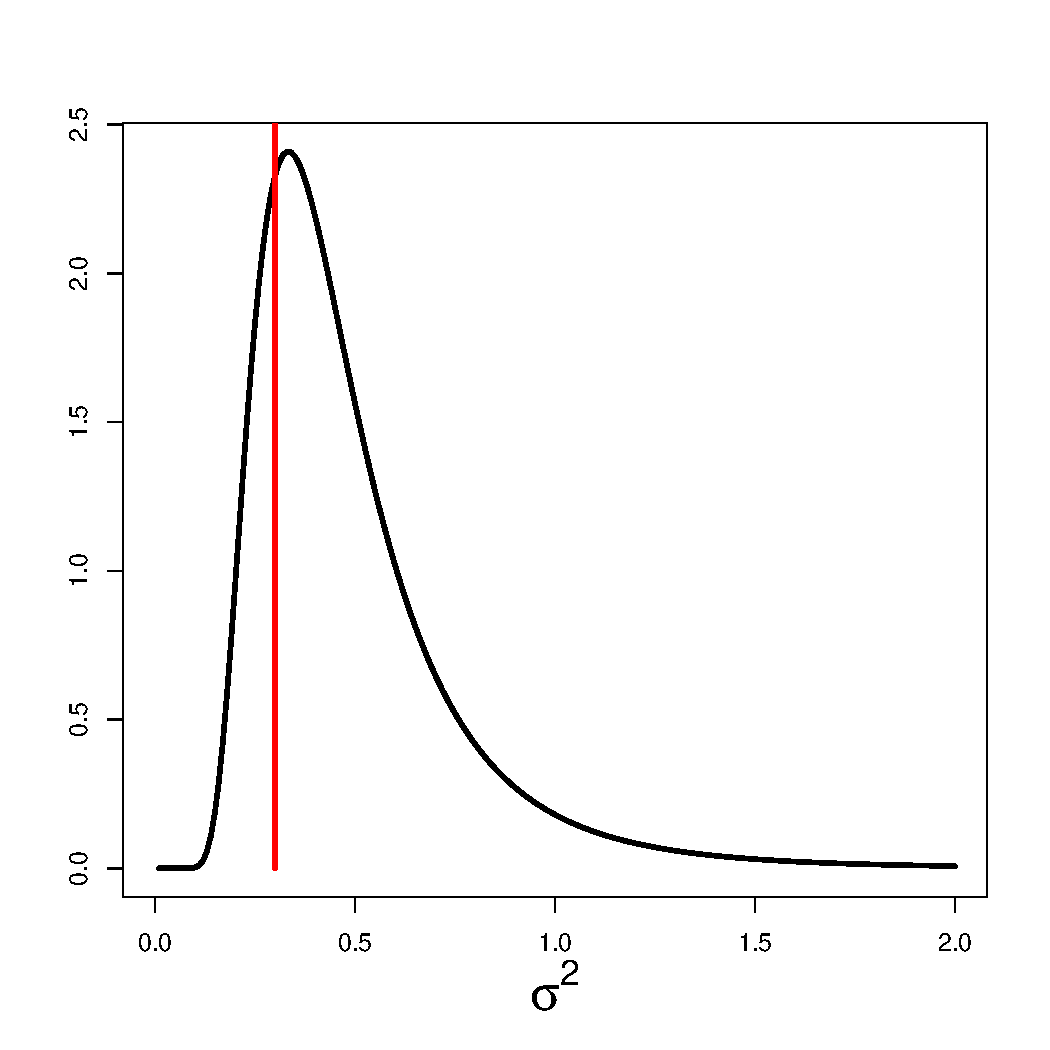
\includegraphics[scale=.2]{priorsig2.pdf}
  \item Gibbs algorithm to simulate couples $(\btheta,\sigma^2)$ from $\pi(\btheta,\sigma^2|\byexp)$.
  Iterate :
  \begin{enumerate}
   \item MH algorithm to simulate $\btheta_{t}$ from $\pi(\cdot|\byexp,\sigma^2_{t-1})$,
   \item conditional simulation of $\sigma^2_{t}$ from $\pi(\cdot|\byexp,\btheta_{t})$.
  \end{enumerate}

  \end{itemize}

 
\end{frame}


\begin{frame}
 \frametitle{Posterior distributions}
 
 \begin{figure}
  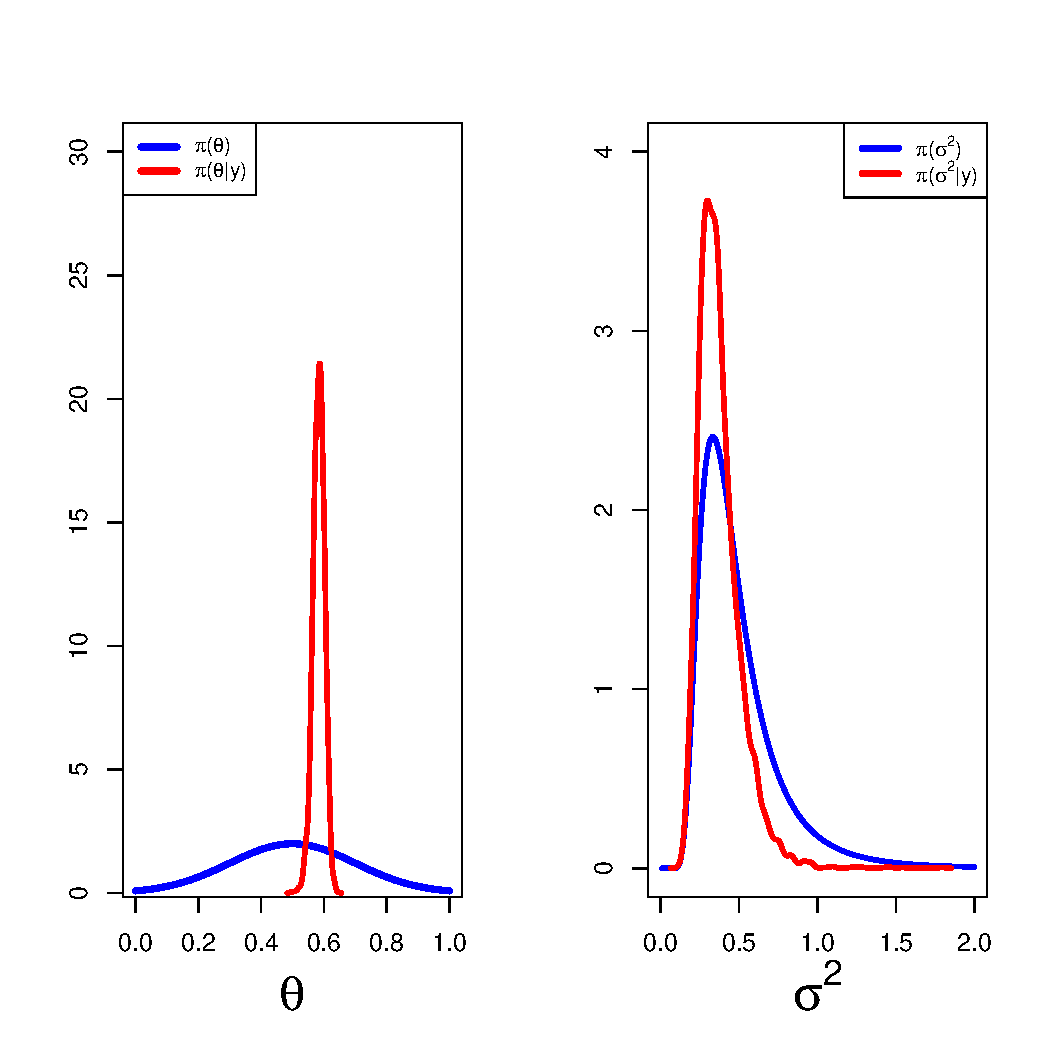
\includegraphics[scale=.4]{calibsig2inconnu.pdf}
 \end{figure}

 
\end{frame}


\begin{frame}
 \frametitle{Comparison}
 
 \begin{figure}
  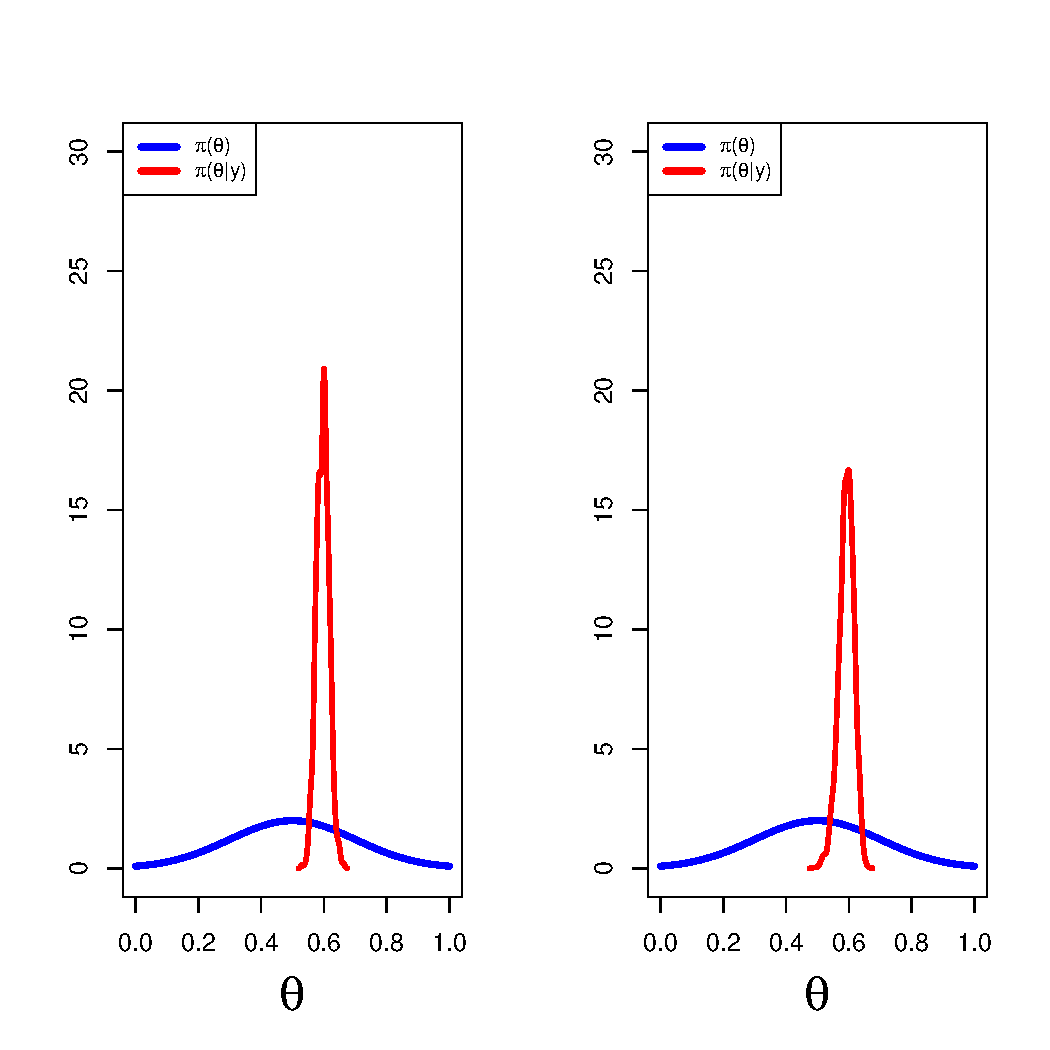
\includegraphics[scale=.35]{calibcomparsig2incouconnu.pdf}
  \caption{known $\sigma^2$ vs unknown $\sigma^2$}
 \end{figure}
\end{frame}



 \section{More complex models}

\begin{frame}
 \frametitle{Relationship between the simulator and the data}

 for $i=1,\ldots, n$,
\begin{itemize}
 \item if the simulator  represents sufficiently well the physical system:
 \begin{equation*}
  \label{nodisc}
 \yexpi=f(\bxexp_i,\btheta^*)+\epsilon(\bxexp_i)\,,
 \end{equation*}
 i.e. for the unknown value $\btheta=\btheta^*: f(\bx,\theta^*)=\zeta(\bx) $ for any $\bx\in \mathcal{X}$,

 \item if the field observations are inconsistent with the simulations (irreducible model discrepancy):
 \begin{equation*}
  \label{disc}
 \yexpi=f(\bx_i,\btheta^*)+\delta(\bx_i) +\epsilon(\bx_i)\,.
 \end{equation*}
 $\delta(\cdot)$ models the difference between the simulator and the physical system:
 $$\delta(\bx)=\zeta(\bx)-f(\bx,\theta^*) \,.$$
\end{itemize}

 
\bigskip

\begin{beamerboxesrounded}{Limited computational budget:}
 Limited number $M$ of runs of the simulator.
\end{beamerboxesrounded}

 

 Ref.:
\cite{kennedy2001,higdon2004}
 \end{frame}




% \begin{frame}
%  \frametitle{Statistical model}
%  \begin{eqnarray}
% \mathcal{M}_3 \ : \ \forall i \in \llbracket 1,\dots,n\rrbracket \quad y_{exp_i}&=& f_c(\boldsymbol{x}_i,\btheta)+\delta(\boldsymbol{x}_i)+\epsilon_i,
% \label{eq:M3}\\
% \delta(\bullet) & \sim &{\GP}{\Big(\boldsymbol{m}_{\delta}(\bullet),c_{\delta}(\bullet,\bullet)\Big)},
% \nonumber
% \end{eqnarray}
%  
% \end{frame}





\begin{frame}
 \frametitle{Statistical models}
 
 
 \begin{align*}
\mathcal{M}_0 : & \ \forall i \in \llbracket1,\dots,\nexp\rrbracket \quad \yexpi=\zeta(\bxexp_i)+\epsilon_i\\
\mathcal{M}_1 :& \ \forall i \in \llbracket1,\dots,\nexp\rrbracket \quad  \yexpi=f_c(\bxexp_i,\btheta)+\epsilon_i,\\
\mathcal{M}_2  :& \ \forall i \in \llbracket1,\dots,\nexp\rrbracket \quad \yexpi = F(\bxexp_i,\btheta) + \epsilon_i,\\
\mathcal{M}_3  :&  \ \forall i \in \llbracket1,\dots,\nexp\rrbracket \quad \yexpi= f_c(\bxexp_i,\btheta)+\delta(\bxexp_i)+\epsilon_i,\\
\mathcal{M}_4  : &\ \forall i \in \llbracket1,\dots,\nexp\rrbracket \quad \yexpi= F(\bxexp_i,\btheta)+\delta(\bxexp_i)+\epsilon_i.
\end{align*}

where 
\begin{itemize}
 \item $\epsilon_i\overset{iid}{\sim} \mathcal{N}(0,\sigma_{err}^2)$,
 \item $F(\bullet,\bullet)  \sim{\GP}{\Big(m_S(\bullet,\bullet),c_S\{(\bullet,\bullet),(\bullet,\bullet)\}\Big)},$ on $\mathbb{X}\times \Theta$
 \item 
$\delta(\bullet)  \sim {\GP}{\Big(\boldsymbol{m}_{\delta}(\bullet),c_{\delta}(\bullet,\bullet)\Big)}$ on $\mathbb{X}$.
\end{itemize}

 \cite{carmassi2019bayesian}
 
\end{frame}


\begin{frame}
 \frametitle{Likelihood for $\mathcal{M}_1$ and $\mathcal{M}_3$}
 
 
 \begin{equation*}
\begin{split}
\mathcal{L}^{F}(\btheta,\boldsymbol{\beta}_{\delta},\Phi_{\delta};\byexp,\bXexp)=\frac{1}{(2\pi)^{\nexp/2}|\boldsymbol{V}_{exp}(\bXexp)|^{1/2}}\exp\Bigg\{-\frac{1}{2}\Big(\byexp-\boldsymbol{m}_{exp}(\bXexp,\btheta)\Big)^T\boldsymbol{V}_{exp}(\bXexp)^{-1}\\
\Big(\byexp-\boldsymbol{m}_{exp}(\bXexp,\btheta)\Big)\Bigg\}.
\end{split}
\label{eq:LikelihoodQuick2}
\end{equation*}
 
\begin{equation*}
\mathbb{E}[\byexp|\btheta,\boldsymbol{\beta}_{\delta};\bXexp] = \boldsymbol{m}_{exp}^{\boldsymbol{\beta}_{\delta}}(\bXexp,\btheta) = \boldsymbol{m}_{exp}(\bXexp,\btheta) = f_c(\bXexp,\btheta) + {\color{gray} {\boldsymbol{H}_{\delta}}(\bXexp)\boldsymbol{\beta}_{\delta}}.
\end{equation*}

Then, the expression of the variance is given by

\begin{equation*}
\mathbb{V}ar[\byexp|\Phi_{\delta};\bXexp] = \boldsymbol{V}_{exp}^{\Phi_{\delta},\sigma_{err}^2}(\bXexp)= \boldsymbol{V}_{exp}(\bXexp) = \boldsymbol{\Sigma}_{\delta}(\bXexp) + \sigma_{err}^2\boldsymbol{I}_{\nexp},
\end{equation*}


with $\forall (i,j) \in \llbracket1,\dots,n\rrbracket^2: (\boldsymbol{\Sigma}_{\delta}(\bXexp))_{i,j} =(\boldsymbol{\Sigma}^{\Phi_{\delta}}_{\delta}(\bXexp))_{i,j}=\sigma^2_{\delta} c_{\delta}(\{\boldsymbol{x}_i,\boldsymbol{x}_j\})$.


\bigskip

\begin{beamerboxesrounded}{For $\mathcal{M}_1$}
 $\boldsymbol{m}_{exp}(\bXexp,\btheta)= f_c(\bXexp,\btheta)$ and $\boldsymbol{V}_{exp}(\bXexp)=\sigma_{err}^2\boldsymbol{I}_{\nexp}$.
\end{beamerboxesrounded}

\end{frame}




\begin{frame}
 \frametitle{When the code is slow}

\textbf{Data:}

\begin{enumerate}
 \item DoNE: Design of Numerical Experiments: $\Dc=\{(\bx_1,\btheta_1),\ldots,(\bx_N,\btheta_N)\}$  %(space-filling or optimize with respect to a given goal: rare event, global optimization)
with corresponding evaluations of the computer model (time-consuming):
$$\byc=f(\Dc)=\{f(\bx_1,\btheta_1),\ldots,f(\bx_N,\btheta_N)\}\,.$$
 
 
 \item DoFE: Design of Field Experiments: $\bXexp=\{\bxf_1,\ldots,\bxf_{\nexp}\}$ with corresponding noisy observation of $\zeta$:$$\byf=\{\yexp_1=\zeta(\bxf_1)+\epsilon_1,\ldots,\yexp_{\nexp}=\zeta(\bxf_{\nexp})+\epsilon_{\nexp}\}\,.$$
\end{enumerate}

\smallskip

\textbf{Model:}\quad
$\forall 1\le i \le \nexp,\quad \yexpi = f(\bxf_i,\btheta) + \delta(\bxf_i) +\epsilon_i$
where:

\smallskip
\begin{itemize}
 \item $f$ is emulated via a GP Emulator \cite{sacks1989} : $f\sim \GP(m_S(\cdot),\sigma_S^2C_S(\cdot,\cdot))$,\\ $f|f(\Dc)\sim \GP$ is the emulator/surrogate/metamodel,
 \item $\delta$ the discrepancy modeled as a GP: $\delta\sim \GP(H_\delta(\cdot)\bbeta_{\delta},\sigma_\delta^2C_\delta(\cdot,\cdot))$,
 \item $\epsilon\overset{iid}{\sim}\mathcal{N}(0,\sigma_{err}^2)$ are measurement errors.
\end{itemize}



\end{frame}


\begin{frame}
 \frametitle{Likelihood for $\mathcal{M}_2$ and $\mathcal{M}_4$}

 $\Phi=(\sigma^2_c,\phi_c,\sigma^2_{\delta},\phi_\delta)$, and $\bbeta=(\bbeta_S,\bbeta_\delta)$\\
 
 Full Likelihood written for $\by=(\byf,\byc)$:
 
 \begin{equation*}
\begin{split}
&\mathcal{L}^F(\btheta,\boldsymbol{\beta},\Phi,\sigma_{err}^2;\boldsymbol{y},\bXexp,\Dc)\\=&\frac{1}{(2\pi)^{(\nexp+N)/2}|\boldsymbol{V}((\bXexp,\btheta),\Dc)|^{1/2}}\\
&\exp\Bigg\{-\frac{1}{2}\Big(\boldsymbol{y}-\boldsymbol{m}_{\boldsymbol{y}}((\bXexp,\btheta),\Dc)\Big)^T
\boldsymbol{V}((\bXexp,\btheta),\Dc)^{-1}
\Big(\boldsymbol{y}-\boldsymbol{m}_{\boldsymbol{y}}((\bXexp,\btheta),\Dc)\Big)\Bigg\}.
\end{split}
\label{eq:FullLikelihood}
\end{equation*}

with 

 \begin{equation*}
\begin{split}
\mathbb{E}[\boldsymbol{y}|\btheta,\boldsymbol{\beta};\bXexp,\Dc]=\boldsymbol{m}_{\boldsymbol{y}}^{\boldsymbol{\beta}}((\bXexp,\btheta),\Dc) =& \boldsymbol{m}_{\boldsymbol{y}}((\bXexp,\btheta),\Dc) =\boldsymbol{H}((\bXexp,\btheta),\Dc)\boldsymbol{\beta}\\&=\begin{pmatrix}
\boldsymbol{H}_S(\bXexp,\btheta) & {\color{gray}\boldsymbol{H}_{\delta}(\bXexp)}\\
\boldsymbol{H}_S(\Dc) & 0
\end{pmatrix}\begin{pmatrix}
\bbeta_S \\ \bbeta_\delta
\end{pmatrix}
.
\end{split}
\label{eq:MeanFullLikelihood}
\end{equation*}
\begin{equation*}
\begin{split}
\mathbb{V}ar[\boldsymbol{y}|\btheta,\Phi,\sigma_{err}^2;\bXexp,\Dc]&=\boldsymbol{V}^{\Phi,\sigma_{err}^2}((\bXexp,\btheta),\Dc)=\boldsymbol{V}((\bXexp,\btheta),\Dc)\\&=\begin{pmatrix}
 \boldsymbol{\Sigma}_{exp,exp}(\bXexp,\btheta) +\boldsymbol{\Sigma}_{\delta}(\bXexp) +\sigma_{err}^2\boldsymbol{I}_{\nexp} &  \boldsymbol{\Sigma}_{exp,c}((\bXexp,\btheta),\Dc)\\
 \boldsymbol{\Sigma}_{exp,c}((\bXexp,\btheta),\Dc)^T & \boldsymbol{\Sigma}_{c,c}(\Dc)
\end{pmatrix}
\end{split}
\label{eq:VarianceFullLikelihood}
\end{equation*}



\end{frame}


\begin{frame}
 
  \begin{itemize}
\item $\forall (i,j) \in \llbracket1,\dots,\nexp\rrbracket^2: (\boldsymbol{\Sigma}_{exp,exp}(\bXexp,\btheta))_{i,j}=c_S\{(\bxexp_i,\btheta),(\bxexp_j,\btheta)\}$,

\medskip
\item $\forall (i,j) \in \llbracket1,\dots,\nexp\rrbracket\times\llbracket1,\dots,N\rrbracket: (\boldsymbol{\Sigma}_{exp,c}((\bXexp,\btheta),\Dc))_{i,j}=c_S\{(\bxexp_i,\btheta),(\bx_j,\btheta_j)\}$,

\medskip
\item $\forall (i,j)\in\llbracket1,\dots,\nexp\rrbracket^2: (\boldsymbol{\Sigma}_{\delta}(\bXexp))_{i,j}=c_{\delta}\{(\bxexp_i,\bxexp_j)\}$,

\medskip
\item $\forall (i,j)\in \llbracket1,\dots,N\rrbracket^2: (\boldsymbol{\Sigma}_{c,c}(\Dc))_{i,j}=c_S\{(\bx_i,\btheta_i),(\bx_j,\btheta_j)\}$. \newline
\end{itemize}
 
\end{frame}


\begin{frame}
 \frametitle{For $\mathcal{M}_2$}
 Mean 
 \begin{equation*}
\mathbb{E}[\boldsymbol{y}|\btheta,\boldsymbol{\beta}_S;\bXexp,\Dc]=\boldsymbol{m}_{\boldsymbol{y}}((\bXexp,\btheta),\Dc)=\boldsymbol{H}((\bXexp,\btheta),\Dc)\boldsymbol{\beta}_S=\begin{pmatrix}
\boldsymbol{H}_S(\bXexp,\btheta)\\
\boldsymbol{H}_S(\Dc)
\end{pmatrix}\boldsymbol{\beta}_S
\label{eq:MeanFullLikelihood2}
\end{equation*}


\bigskip
and the covariance

\begin{equation*}
\begin{split}
\mathbb{V}ar[\boldsymbol{y}|\btheta,\Phi,\sigma_{err}^2;\bXexp,\Dc]=&\boldsymbol{V}((\bXexp,\btheta),\Dc)=\\
&\begin{pmatrix}
\boldsymbol{\Sigma}_{exp,exp}(\bXexp,\btheta) +\sigma_{err}^2\boldsymbol{I}_{\nexp} & \boldsymbol{\Sigma}_{exp,c}((\bXexp,\btheta),\Dc)\\
\boldsymbol{\Sigma}_{exp,c}((\bXexp,\btheta),\Dc)^T & \boldsymbol{\Sigma}_{c,c}(\Dc)
\end{pmatrix}
\label{eq:VarianceFullLikelihood1}
\end{split}
\end{equation*}
 
\end{frame}





\begin{frame}
 \frametitle{Modularization}
 Advocated in \cite{liu2009}.
 \begin{itemize}
  \item From $\byc$, compute the GP emulator from the partial Likelihood $\mathcal{L}^M(\boldsymbol{\beta}_S,\Phi_S;\byc,\Dc)$,
  \item Plug the GP emulator in the conditional Likelihood of $\byf$: $ \mathcal{L}^C(\btheta,\boldsymbol{\beta}_{\delta},\Phi_{\delta};\boldsymbol{\beta}_S,\Phi_S,\byexp|\byc,\bXexp,\Dc)$.
 \end{itemize}

 
 \bigskip
 
 \cite{gramacy2020surrogates}
 ``Modularization or Compartmentalization is an engineering practice such that Components should perform robustly in isolation, irrespective of their anticipated role in a larger system.''
 
\end{frame}



\begin{frame}
 \frametitle{MLE estimates}
 
 
MLE for $\boldsymbol{\beta}_S,\Phi_S$ from the partial likelihood:
\begin{equation*}
\begin{split}
&\mathcal{L}^M(\boldsymbol{\beta}_S,\Phi_S;\byc,\Dc)\\
&=\frac{1}{(2\pi)^{N/2}|\boldsymbol{V}_c(\Dc)|^{1/2}}\exp\Bigg\{-\frac{1}{2}\Big(\byc-\boldsymbol{m}_c(\Dc)\Big)^T\boldsymbol{V}_c(\Dc)^{-1}\Big(\byc-\boldsymbol{m}_c(\Dc)\Big)\Bigg\}.
\label{eq:PartialLikelihood}
\end{split}
\end{equation*}

\begin{equation*}
\mathbb{V}ar[\byc|\Phi_S;\Dc] = \boldsymbol{V}_c^{\Phi_S}(\Dc)=\boldsymbol{V}_c(\Dc)= \boldsymbol{\Sigma}_{c,c}(\Dc),
\end{equation*}


$$\mathbb{E}[\byc|\boldsymbol{\beta}_S;\Dc]=\boldsymbol{m}_c(\Dc) ={\boldsymbol{H}_S}(\Dc)\boldsymbol{\beta}_S\,.$$
 
 \end{frame}
 
 
 
 \begin{frame}
 \frametitle{GP emulation}
 
 We derive
 \begin{equation*}
\byexp|\byc\sim\mathcal{N}(\boldsymbol{\mu}_{exp|c}((\bXexp,\btheta),\Dc),\boldsymbol{\Sigma}_{exp|c}((\bXexp,\btheta),\Dc))
\end{equation*}
with

\begin{equation*}
\begin{split}
&\boldsymbol{\mu}_{exp|c}((\bXexp,\btheta),\Dc)\\
&= {\boldsymbol{H}_S}(\bXexp,\btheta) \boldsymbol{\beta}_S + {\boldsymbol{H}_{\delta}}(\bXexp)\boldsymbol{\beta}_{\delta}+\boldsymbol{\Sigma}_{exp,c}((\bXexp,\btheta),\Dc)\boldsymbol{\Sigma}_{c,c}(\Dc)^{-1}(\byc-\boldsymbol{m}_c(\Dc)),
\label{eq:conditionnalMean}
\end{split}
\end{equation*}

\bigskip
\begin{equation*}
\boldsymbol{\Sigma}_{exp|c}((\bXexp,\btheta),\Dc)=\boldsymbol{V}_{exp,exp}(\bXexp,\btheta)-\boldsymbol{\Sigma}_{exp,c}((\bXexp,\btheta),\Dc)\boldsymbol{\Sigma}_{c,c}(\Dc)^{-1}\boldsymbol{\Sigma}_{exp,c}((\bXexp,\btheta),\Dc)^T,
\label{eq:conditionnalVariance}
\end{equation*}
 
 with 
 
 $\boldsymbol{V}_{exp,exp}(\bXexp,\boldsymbol{\theta})=\boldsymbol{\Sigma}_{exp,exp}(\bXexp,\boldsymbol{\theta})+\boldsymbol{\Sigma}_{\delta}(\bXexp) +\sigma_{err}^2\boldsymbol{I}_{\nexp}.$
 
\end{frame}


\begin{frame}
 \frametitle{GP emulator illustrated}
 \centering
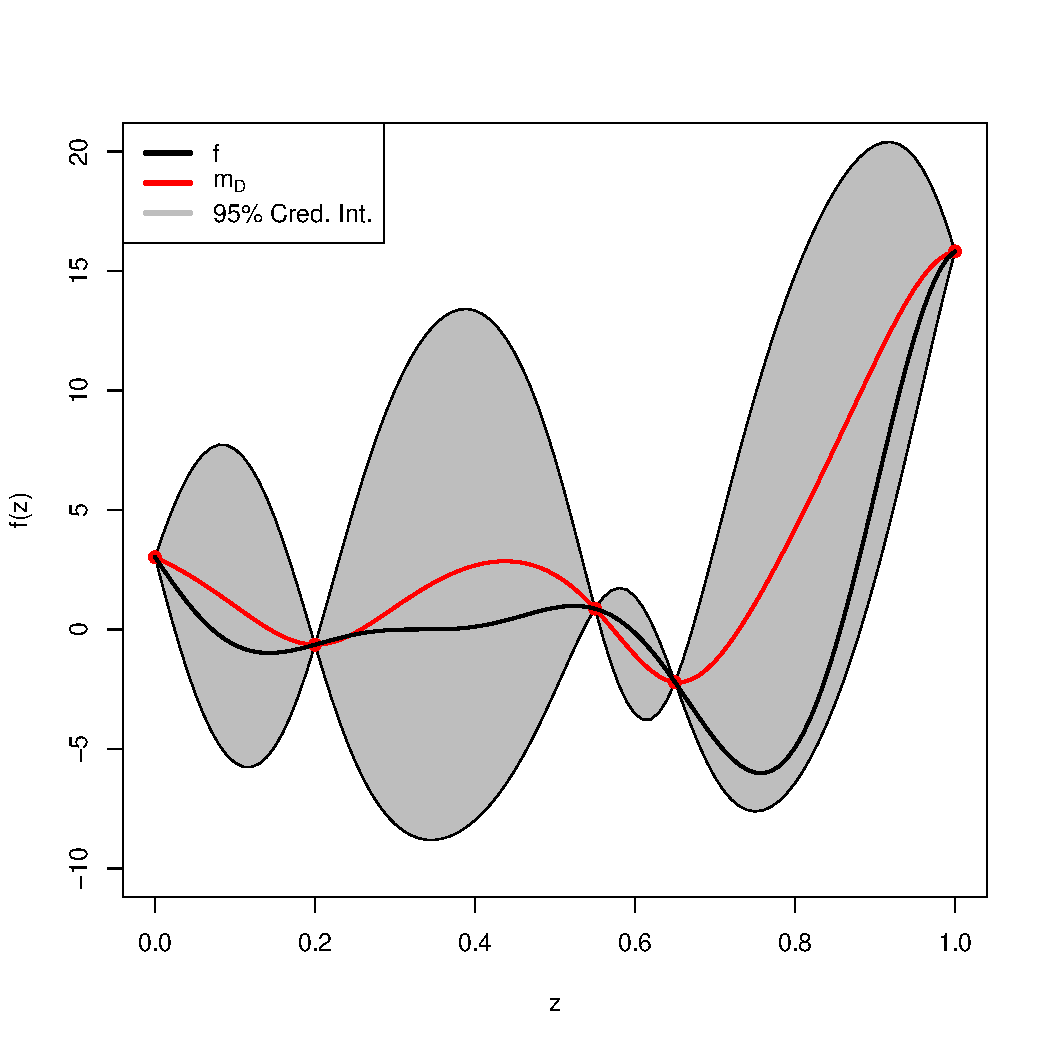
\includegraphics[scale=.3]{exkriging.pdf}

\end{frame}



\begin{frame}
 \frametitle{Conditional Likelihood}
 GP emulator plugged into 
 
 \begin{equation*}
\begin{split}
&\mathcal{L}^C(\btheta,\boldsymbol{\beta}_{\delta},\Phi_{\delta},\sigma^2_{err};\hat{\boldsymbol{\beta}_S},\hat{\Phi_S},\byexp|\byc,\bXexp,\Dc)\\ \propto &|\Sigma_{exp|c}((\bXexp,\btheta),\Dc)|^{-1/2}\\ &\exp\Big\{-\frac{1}{2}(\byexp-\mu_{exp|c}((\bXexp,\btheta),\Dc))^T \Sigma_{exp|c}((\bXexp,\btheta),\Dc)^{-1} (\byexp-\mu_{exp|c}((\bXexp,\btheta),\Dc))\Big\}.
\label{eq:conditionalLikelihood}
\end{split}
\end{equation*}
 
\end{frame}


\begin{frame}
 \frametitle{Frequentist estimation: least squares estimation}
 \cite{cox2001,wong2017}
 \begin{equation}
\hat{\btheta}= \underset{\btheta\in\mathcal{Q}}{argmin} \ M_n(\btheta) \quad \text{with} \quad M_n(\btheta)=\frac{1}{\nexp}\sum_{i=1}^{\nexp} \{\yexp_i-f(\bxexp_i,\btheta)\}^2,
\end{equation}

and \\
estimation of $\delta_0$  applying any nonparametric regression method to the “data”
$$\{\bx_i, \yexpi - f(\bxexp_i,\hat\btheta)\}_{i=1,\ldots,\nexp}.$$


\end{frame}



\begin{frame}
 \frametitle{Bayesian estimation for $\mathcal{M}_4$}
 \textbf{Prior information:} \begin{equation*}
\pi(\btheta,\boldsymbol{\beta},\Phi,\sigmaerr) = \pi(\btheta) \times 1 \times \pi(\Phi)\times \pi(\sigmaerr).
\label{eq:PriorDistribution}
\end{equation*}


\textbf{Estimation}


\begin{itemize}
 \item Full Bayesian: 
For a full Bayesian analysis, integrating other parameters out is needed to finally get $\pi(\btheta|\boldsymbol{y})$,
\item Modular: 
\begin{enumerate}
 \item maximizing the likelihood $\mathcal{L}^M(\boldsymbol{\beta}_S,\Phi_S|\byc;\Dc)$  to get the maximum likelihood estimates (MLE) $\hat{\boldsymbol{\beta}}_S$ and $\hat{\Phi}_S$ of $\boldsymbol{\beta}_S$ and $\Phi_S$
 \item plugged into the conditional likelihood $\mathcal{L}^C(\btheta,\boldsymbol{\beta}_{\delta},\Phi_{\delta},\sigmaerr; \hat{\boldsymbol{\beta}}_S,\hat{\Phi_S},\byexp|\byc,\bXexp,\Dc)$
 \item  sampled with MCMC methods:\\ $\pi(\btheta,\boldsymbol{\beta}_\delta,\Phi_\delta,\sigmaerr|\byexp,\byc,\bXexp,\Dc)\propto  \mathcal{L}^C(\btheta,\boldsymbol{\beta}_{\delta},\Phi_{\delta},\sigmaerr;\hat{\boldsymbol{\beta}}_S,\hat{\Phi_S},\byexp|\byc,\bXexp,\Dc)\cdot \pi(\btheta,\boldsymbol{\beta}_\delta,\Phi_\delta,\sigmaerr)$
\end{enumerate}

\item Generate explicitely realizations of $(\delta(\bx_i))_{1\le i\le \nexp}$ conditionally on the current parameters values in a Gibbs sampling algorithm.
\cite{bayarri2007}.% computationally demanding since simulation from a GP 


\end{itemize}


\end{frame}



\begin{frame}
 \frametitle{for other models}
 For $\mathcal{M}_1$ and $\mathcal{M}_3$ no modularization use the actual code in the likelihood.
 
 
 
\end{frame}





% \begin{frame}
%  \frametitle{MCMC algorithms}
%  
%  technical details???
%  
% \end{frame}
% 

\section{Additional comments}
\begin{frame}
 \frametitle{A word on history matching}
 
 
 \begin{itemize}
  \item common alternative to KOH calibration \cite{craig1997pressure,vernon2010galaxy, Boukouvalas2014Calibration, Andrianakis2017efficient}.
  \item searches for inputs where the simulator outputs closely match observed data, while recognizing the presence of the various uncertainties, including model discrepancy
  \item rules out ``implausible'' inputs,
  
 \end{itemize}

$\btheta$ is deemed implausible if:
\begin{equation}
\frac{||\yexp - f(\bxexp,\btheta)||}{\sqrt{\sigma^2_S(\bxexp,\btheta) + \sigma^2_{\delta}(\bxexp) + \sigmaerr)}} \geq 3,
\label{eq:eqhm}
\end{equation}
where $\sigma^2_S, \sigma^2_{\delta}$, and $\sigmaerr$ are the variances of the surrogate, the model discrepancy, and the observational error.


\begin{itemize}
 \item number 3 comes from \cite{pukelsheim1994three} who shows that at least $95\%$ of any unimodal distribution is contained within three standard deviations,
 \item HM can be repeated in so-called ``waves'', using non-implausible $\btheta$ found at one wave to generate simulation runs for the next wave
\item simulator not valid if plausible space is void.
 \end{itemize}
% 
% In other words, an input is implausible if the difference between the observation and the simulator output (using that input) is sufficiently large relative to those uncertainties. The . When there are multiple outputs or additional, controllable, inputs there are modifications to equation \ref{eq:eqhm} \cite{vernon2010galaxy}. 

% The process , sequentially reducing the space where $u_C$ could lie. With these waves HM, aims to avoid regions of inputs where $u_C$ is unlikely to be and, in that regard, HM is a also calibration design scheme. At any given wave, it is possible for all values of $u_C$ to be deemed implausible — the so-called terminal case  \cite{salter2019uncertainty} — usually implying that $\sigma^2_{\mathrm{MD}}$ is set too low or that the simulator is not fit for purpose.
\end{frame}



\bibliographystyle{apalike}
\bibliography{biblio}





\end{document}
